\documentclass[a4paper,11pt]{article}
\usepackage{physics}
\usepackage{amsmath}
\numberwithin{equation}{section}

\usepackage[qm]{qcircuit}
\usepackage{bibentry}




\usepackage{tikz,tikz-cd}



\usepackage{siunitx}
\usepackage{braket}
\usepackage{authblk}
\usepackage[a4paper, margin=1.5in]{geometry}
\usepackage{parskip}
\setlength{\parindent}{15pt}
\usepackage{tikz}
\usetikzlibrary{arrows, calc, patterns, angles, quotes}
\usetikzlibrary{decorations.pathmorphing}
\usepackage{amssymb}
\usetikzlibrary{shapes.geometric}
\usepackage[section]{placeins}
\usepackage{pgfplots}
\usepackage{clock}
\usepackage[clock]{ifsym}
\usetikzlibrary{shapes}
\usepackage{amsthm}
\theoremstyle{definition}
\newtheorem{thm}{Theorem}[section]
\newtheorem{defn}{Definition}[section]
\newtheorem{prop}{Proposition}[section]
\newtheorem{rmk}{Remark}[section]
\newtheorem{exmp}{Exercise}[section]
\newtheorem*{prob*}{Problem}
\newtheorem{prob}{Problem}[section]
\newtheorem*{sln*}{Solution}
\newtheorem{sln}{Solution}[section]
\usepackage{empheq}
\usepackage{hyperref}
\usepackage{tensor}
\usepackage{xcolor}
\hypersetup{
	colorlinks,
	linkcolor={black!50!black},
	citecolor={blue!50!black},
	urlcolor={blue!80!black}
}
\newcommand{\p}{\partial}
\newcommand{\lag}{\mathcal{L}}
\newcommand{\E}{\mathcal{E}}
\newcommand{\V}{\mathcal{V}}
\newcommand{\nn}{\nonumber}

\newcommand{\f}[2]{\frac{#1}{#2}}

\newcommand{\ift}{\infty}

\newcommand{\lp}{\left(}
\newcommand{\rp}{\right)}

\newcommand{\lb}{\left[}
\newcommand{\rb}{\right]}

\newcommand{\lc}{\left\{}
\newcommand{\rc}{\right\}}
%\usepgfplotslibrary{external}
%\tikzexternalize

\begin{document}
\begin{titlepage}\centering
 \clearpage
 \title{\textsc{\bf{Matrices in Quantum Computing}}\\\smallskip A 2-qubit Entangler Circuit\\}
 \author{\bigskip Huan Q. Bui}
 \affil{Colby College CLAS 2019\\$\,$\\ PHYSICS \& MATHEMATICS\\ Statistics \\$\,$\\Class of 2021\\}
 \date{\today}
 \maketitle
 \thispagestyle{empty}
\end{titlepage}

\newpage

\section{Introduction}

Quantum computing and quantum information science are rapidly growing fields in recent years. Progress is made everyday in not only in the physics labs but also in the mathematical foundation, most of which is linear algebra. The matrix theory behind quantum computing is voluminous, and thus it would be insane for me to talk about all kinds of matrices in quantum computing. So today, I would like to draw your attention to one of the simplest and basic yet interesting circuits in all of quantum computing: the 2-qubit entanglement circuit, and some of the matrix theory behind it. 

\begin{center}
	$\,$\Qcircuit @C=.7em @R=.4em  {
		\lstick{a: \ket{0}} & \qw & \qw & \targ & \meter & \qw \\
		\lstick{b: \ket{0}} & \qw & \gate{H} & \ctrl{-1}& \meter & \qw 
	}
\end{center}

\section{Presentation layout}
Here's my plan for this presentation. I will 
\begin{enumerate}
	\item first provide some background on quantum computing. I will introduce some of the basic objects in quantum computing such as qubits, quantum circuits, quantum gates, and entanglement. 
	\item And as I introduce these objects, the mathematical concepts of the Kronecker product and tensor product will come up, as they are the building blocks of the theory of quantum computation. I will talk about what these matrix theories are, how they work, and, time permitting, ``why'' they are required.
	\item  Then, we will walkthrough the 2-qubit entanglement circuit that I have just shown. We will see how the tensor product appears and how we can use it ``see'' what the circuit actually does.
	\item Finally, I will show how you can actually implement this circuit (or any other circuit) on your browser and have an actual quantum computer at IBM execute the commands.
\end{enumerate}

\section{Qubits}
So let us start with qubits. Qubits are kind of like classical bits, but not really. Classical bits can take values of only 0 and 1, ``on'' or ``off'', ``up'' or ``down,'' while quantum bits can take any ``superposition'' of those two states, since qubits are quantum mechanical objects.

\begin{figure}[h!]
	\centering
	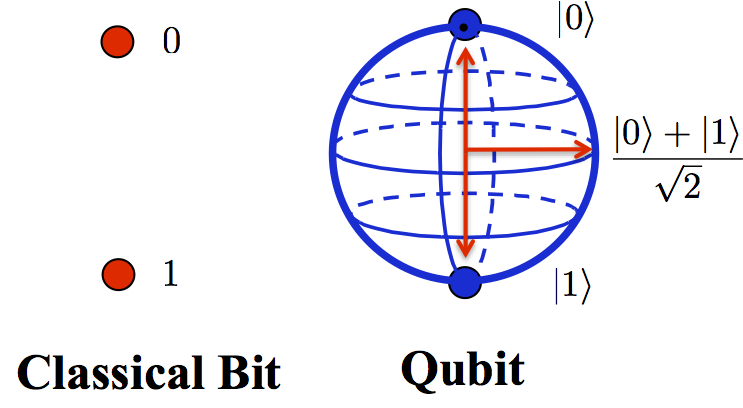
\includegraphics[scale=0.35]{atom1.png}
\end{figure}

Most of the time, qubits are individual atoms that can be excited to the excited state or de-excited into the ground state. Mathematically, we can think of these states as forming a basis for the space of all possible states of the atom, and the state of a qubit can be represented by the following linear combination:
\begin{align*}
a\begin{bmatrix}
1\\0
\end{bmatrix}
+
b\begin{bmatrix}
0\\1
\end{bmatrix},
\end{align*} 
where 
$
\begin{bmatrix}
1\\0
\end{bmatrix} \text{represents the ground state, and}
\begin{bmatrix}
0\\1
\end{bmatrix} \text{represents the excited state}
$. The coefficients $a,b$ are complex numbers such that the sum of the modulus squares is one:
\begin{align*}
\abs{a}^2 + \abs{b}^2 = 1,
\end{align*}
the reason being, in quantum mechanics, it is require that the magnitude of the state vector is 1. In fact, in physics, it is often interpreted that $\abs{a}^2$ is the probability of the qubit being in the ground state, and $\abs{b}$ is the probability of the qubit being in the excited state. 

Now, before we move on, for the sake of convenience, let us introduce a new notation for the basis states of a qubit. Let $\ket{0}$ represent the vector $\begin{bmatrix}
1 & 0
\end{bmatrix}^\top$ and $\ket{1}$ represent the vector $\begin{bmatrix}
0&1
\end{bmatrix}^\top$. The reason for doing this is that now we can just call the ground state the ``zero'' state and excited state the ``one'' state, giving us a nice way to relate the basis values of a classical bit. So, the state of single qubit can be  written as
\begin{align*}
a\ket{0} + b\ket{1}.
\end{align*}



\section{Quantum gates}
Another fundamental object in quantum computing is quantum gates. If we think of states of qubits as vectors, then quantum gates are modeled by linear transformations - matrices - on the state vectors of qubits. For example, one of the most common and important single-qubit quantum gates, is called the Hadamaar gate, which is in matrix form is
\begin{align*}
H = \f{1}{\sqrt{2}}\begin{bmatrix}
1&1\\
1&-1
\end{bmatrix}.
\end{align*}
This gate is actually the first component on the quantum circuit we have seen:
\begin{center}
	$\,$\Qcircuit @C=.7em @R=.4em  {
		\lstick{a: \ket{0}} & \qw & \qw & \targ & \meter & \qw \\
		\lstick{b: \ket{0}} & \qw & \gate{H} & \ctrl{-1}& \meter & \qw 
	}
\end{center}
The Hadamaar gate is denoted with an $H$. We can see what $H$ does to, say $\ket{0}$:
\begin{align*}
H\ket{0} = H\begin{bmatrix}
1\\0
\end{bmatrix} = \f{1}{\sqrt{2}}\begin{bmatrix}
1&1\\1&-1
\end{bmatrix}\begin{bmatrix}
1\\0
\end{bmatrix} = \f{1}{\sqrt{2}}\begin{bmatrix}
1\\1
\end{bmatrix},
\end{align*}
which we can equivalently write as
\begin{align*}
\f{1}{\sqrt{2}}\ket{0} + \f{1}{2}\ket{1}.
\end{align*}
So what the Hadamaar gate does is putting a pure state into a perfect superposition, with exactly 50\% chance of finding the qubit either state $\ket{0}$ or $\ket{1}$. 


\section{Multiple qubits}
Like classical circuits, quantum circuits require multiple qubits to operate. And so a natural question to ask now is how do we represent the quantum state of 2-qubits with the same vector. Let us say that the qubit 1 has state $$a\ket{0} + b\ket{1} = \begin{bmatrix}
a\\b
\end{bmatrix}$$ and qubit 2 has state $$c\ket{0} + d\ket{1} = \begin{bmatrix}
c\\d
\end{bmatrix}.$$ It is clear that we can neither add, nor ``multiply'' these ``pairs'' in any traditional way in order to get a vector of unit length. It turns out that if we do the following seemingly ``magical'' multiplication procedure,
\begin{align*}
\begin{bmatrix}
a\\b
\end{bmatrix}
\boxtimes
\begin{bmatrix}
c\\d
\end{bmatrix} = \begin{bmatrix}
a\begin{bmatrix}
c\\d
\end{bmatrix}\\
b\begin{bmatrix}
c\\d
\end{bmatrix}
\end{bmatrix}
=
\begin{bmatrix}
ac\\ad\\bc\\bd
\end{bmatrix}.
\end{align*}
We can check quite easily that this new vector has unit length. Applying this procedure to the basis states $\ket{0}$, $\ket{1}$, we actually get a basis for the vector space that contains all possible quantum states of two qubits:
\begin{align*}
\ket{0}\boxtimes \ket{0}
=
\begin{bmatrix}
1\\0\\0\\0
\end{bmatrix}, \ket{0}\boxtimes \ket{1}
=
\begin{bmatrix}
0\\1\\0\\0
\end{bmatrix}, \ket{1}\boxtimes \ket{0}
=
\begin{bmatrix}
0\\0\\1\\0
\end{bmatrix}, \ket{1}\boxtimes \ket{1}
=
\begin{bmatrix}
0\\0\\0\\1
\end{bmatrix}, 
\end{align*}
and so it is convenient for us to write
\begin{align*}
\ket{00} = \ket{0} \boxtimes \ket{0}\\
\ket{01} = \ket{0} \boxtimes \ket{1}\\
\ket{10} = \ket{1} \boxtimes \ket{0}\\
\ket{11} = \ket{1} \boxtimes \ket{1}
\end{align*}
where the first slot indicates the (pure) state of the first qubit, and the second slot indicates the (pure) state of the second qubit. And so it is not so hard to see that
\begin{align*}
\begin{bmatrix}
a\\b
\end{bmatrix}
\boxtimes
\begin{bmatrix}
c\\d
\end{bmatrix} = ac\ket{00} + ad\ket{01} + bc\ket{10} + bd\ket{11}. 
\end{align*}

\section{Caveat 1}
With this, we can see that given two qubits with defined states, this ``product'' always gives us a new two-qubit joint state, and we call this joint state \textbf{elementary}. Now, we might wonder whether any joint state can be expressed as this special product of two single-qubit states. It turns out that the answer is no. 

This is a subtle fact. So, let us consider an analogue to this, with polynomials. Let us consider two vectors spaces of polynomials of $x$ and of $y$. It is clear that $p(x)q(y)$ is contained in the vector space of polynomials of both $x$ and $y$. However, this polynomial with both $x$ and $y$,
\begin{align*}
xy + 1,
\end{align*}
cannot be written as a product of a polynomial in $x$ and one in $y$. 

Back to qubits. Consider the following example. This joint state
\begin{align*}
\frac{1}{\sqrt{2}}\begin{bmatrix}
1\\0\\0\\1
\end{bmatrix} = \f{1}{\sqrt{2}}\ket{00} + \f{1}{\sqrt{2}}\ket{11}
\end{align*}
cannot be written as this special product of two single-qubit states. These qubits are now in a state we call \textbf{entanglement}. 

\section{Kronecker product}
similar thing for matrices?


\end{document}